\documentclass[twoside,11pt]{article}

\usepackage{jmlr2e}

\usepackage[utf8]{inputenc}
\usepackage{amsmath, latexsym}
\usepackage{tikz}
\usepackage{xspace}
\usepackage{wrapfig}
\usepackage{xcolor}  % Coloured text etc.
\usepackage[printonlyused,withpage]{acronym}

% For notes
% 
\usepackage[colorinlistoftodos,prependcaption]{todonotes}
%

\acrodef{YOLO}[YOLO]{You Only Look Once}
\acrodef{ALPR}[ALPR]{Automatic License Plate Recognition}
\acrodef{LPCS}[LPCS]{Licence Plate Character Segmentation}
\acrodef{LP}[LP]{Licence Plate}
\acrodef{NN}[NN]{Neural Network}
\acrodef{OCR}[OCR]{Optical Character Recognition}


\firstpageno{1}

\begin{document}

\title{
    Automatic Number-Plate Recognition\\
    Image Processing Group Project Summary\\
    2022/23 Fall Semester
}

\author{\name Barnabás Börcsök
    \email barnabas.borcsok@edu.bme.hu
    \AND
    \name Gergő Haragos
    \email geri.haragos@gmail.com
   \AND
    \name Zoltán Simon
    \email zoltan.simon@edu.bme.hu
   \AND
    \name Bence Sándor Szabó 
    \email szabo.bence.sandor@gmail.com
   \\\vfill\hfill\addr Budapest University of Technology and Economics
}

\maketitle

\section{Introduction}
\todo[inline]{Proofread + Actualize introduction section}

There are many use cases in traffic control, where the \ac{LP} of vehicles must
be read.  This task can be automated by computers. A wall-mounted or even
hand-held camera can take pictures of cars. The image then can be processed by
various algorithms to detect the \ac{LP}, segment the characters and finally
recognise these characters.  In recent years with the increasing amount of
traffic, the need for well-performing \ac{ALPR} systems has increased
substantially.

We propose our own \ac{ALPR} implementation.  We write about the
state-of-the-art literature of the field. Our solution will be based on some of
these publications. Our goal when selecting from the many available methods was
to select the methods with the most promising test results.

We provide a project outline describing our planned tasks. The development
process can be split up into a few large portions. This is visualised on a Gantt
chart, where you can review each subtask.

After successful implementation, we will test our work on predefined training
data as well as further real-life data. We also list some evaluation
considerations.

Our implementation at \url{https://github.com/bobarna/bme-image-processing},
with detailed, reproducable steps.

\todo[inline]{Add document outline here.}


\csection{Previous Solutions}
\label{previous-solutions}

\subsection{Automatic Number-Plate Recognition}
\label{previous-solutions-anpr}
% Section label
In the past years many research projects have been focused on \ac{ALPR}.
We have surveyed some of the most recent and most promising works in this field.
A recent survey by \cite{survOnMet} gives an overview of different methods and
practices used in \ac{ALPR}.

Texture-based methods use characters present on the \ac{LP} as the basis for
\ac{ALPR}. Significant color difference between the board and its characters
creates a high-frequency color transition. If the image is grayscale,
there is an easy to distinguish change of colors between the characters and the
background of the board. This creates a unique pixel intensity distribution in
the region of the plate. The plate region should have a high edge density. This
is used in edge-based systems. In \cite{HongFuJiaHuan} the authors used
scan-line technique for \ac{ALPR}.

Introduced by \cite{redmon2016look} as a novel object detection method,
\ac{YOLO} serves as the basis for the \ac{ALPR} introduced by
\cite{DBLP:journals/corr/abs-1909-01754}.
The naming of \ac{YOLO} comes from the fact that it performs the object detection
for the full image in a single pass. The employed \ac{NN} divides the image
into regions and predicts bounding boxes and probabilities for each region.
Building on this method the authors achieved a license plate recognition rate of
$96.9\%$.  The method was tested on multiple different datasets with outstanding
results.  Besides the novel approach, the authors of this work also released
a public dataset of $38,351$ manually labeled bounding boxes on $6,239$ images.

A benchmark for \ac{ALPR} is introduced by
\cite{DBLP:journals/corr/GoncalvesSMS16}. This benchmark is
composed of a dataset helping the \ac{LPCS} step. High success rate of this step
is crucial for end-to-end success of \ac{ALPR}. Besides the dataset, the authors
also propose a new evaluation measure of the location of the bounding
box within the ground-truth annotation. To further optimise the \ac{LPCS} step,
they suggest a more straightforward approach to perform it efficiently.

\subsection{Optical Character Recognition}
\label{previous-solutions-ocr}
\todo[inline]{Write OCR previous solutions section (Zoli's excellent
notebook is a good starting point)}


\section{Method}
\label{method}
In this section we discuss the different methods used in our solution.  We
deconstruct the task of license plate recognition into arbitrary smaller parts.
The first great challenge of license plate recognition is determining the
location of the plate in the picture.  In an upcoming subsection we will
introduce the used bounding box detection system.  The other major challenge of
license plate recognition is actually reading the plate.  After we have assigned
a bounding box the rest is up to an \ac{OCR} subsystem.  An \ac{OCR} recognises
characters printed on the plate.

%--------------------------------------------------
\subsection{Optical~Character~Recognition}
\label{subsec:ocr}
%--------------------------------------------------

In this subsection we discuss the implementation details of the used \ac{OCR} pipeline.
Our work is based on the paper proposed by Shi et al. \cite{7801919}.
\begin{figure}
	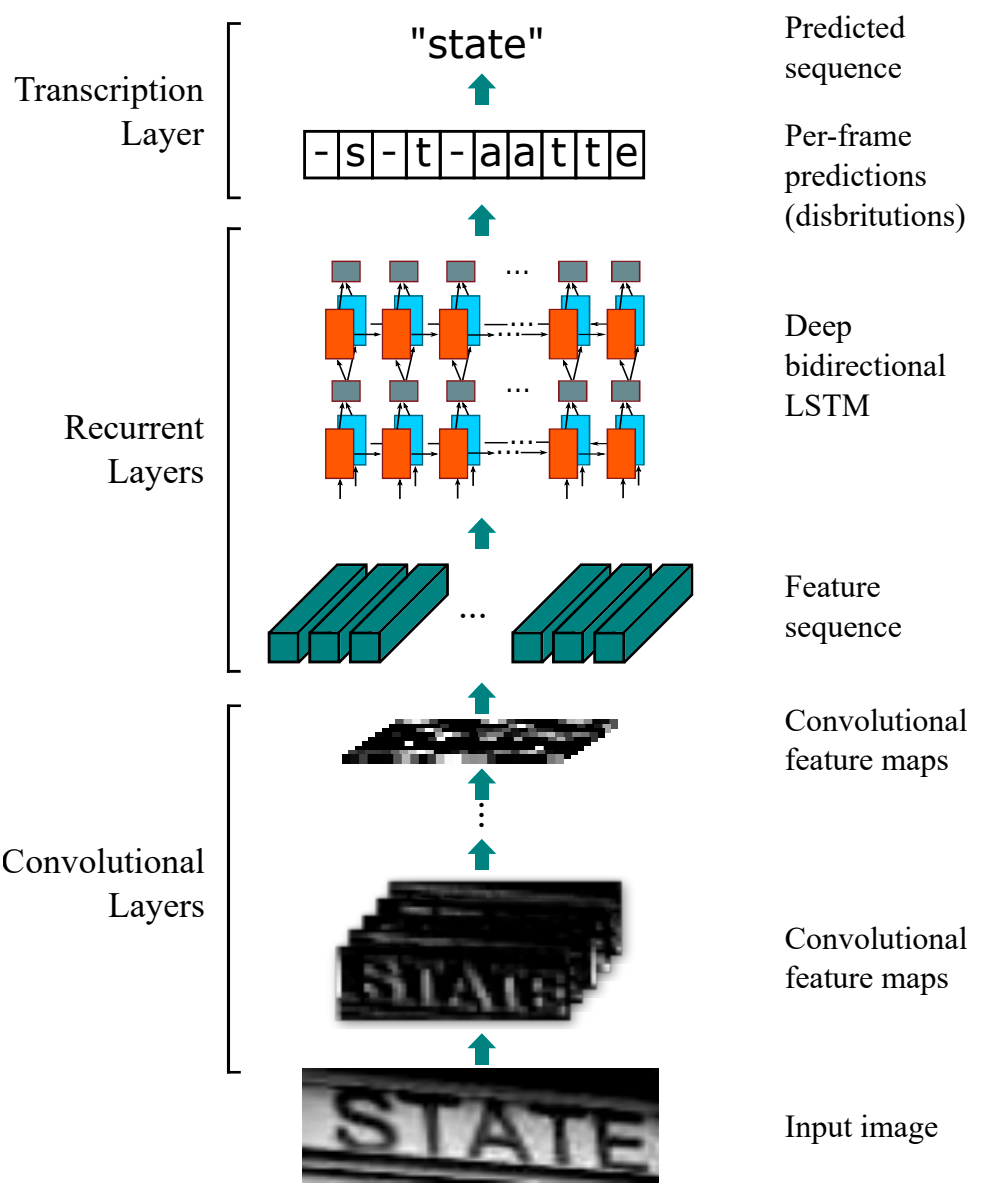
\includegraphics[width=\textwidth]{figures/crnn.png}
	\caption{The architecture published in \cite{7801919}}
	\label{fig:ocr_architecture}
\end{figure}

We deal with the classic problem of computer vision, image-based sequence
recognition. Serial objects, such as scene text, are usually recognized as
a sequence of tags rather than a single tag. RNNs can be trained and optimized
end-to-end, but require complex post-processing steps before being used. CRNN is
a combination of DCNN and RNN and forms an end-to-end system for sequence
recognition. It can be learned directly from sequence labels, does not require
detailed annotations (such as words), and only requires height normalization in
the training and testing sessions.

A CRNN is a type of Recurrent Neural Network (RNN) that can be trained to make
a prediction for each frame of a sequence of features that is output by
convolutional layers. In CRNN, each column of the field maps corresponds to
a region of a rectangle (called the receptive field) of the original image, and
the regions are in the same order as the corresponding columns in the feature
maps from left to right. A deep bidirectional recurrent neural network (CRNN) is
built on top of convolutional layers as recurrent layers.

The recurrent layers predict a label distribution yt for each frame xt of the
feature sequence. Each time it receives a frame in the sequence, it updates its
internal state with a non-linear function that takes both the current input
state and the past state as input. Long-Short-Term Memory (LSTM) is a type of
RNN designed to capture long-range dependencies that often occur in image-based
sequences. LSTM consists of a memory cell and three multiplicative gates, namely
input, output and forget gates. It has made a huge improvement in its speech
recognition function.  Transcription is a process that produces frame-by-frame
predictions into a tag sequence using RNN. Each input in CTC is a sequence
y = y1, ... , yT, where T is the length of the sequence.

We have developed a neural network that can be trained end-to-end on pairs of
images, eliminating the manual labeling of individual components on the training
images. The network is trained with error differences calculated using the
backpropagation algorithm and stochastic gradient descent (SGD).  CRNN is not
limited to recognizing a word in a known dictionary and can handle random
strings ,sentences or other scripts.  The recognition accuracy is plotted as
a function of d. A larger d results in more candidates, thus a more accurate
lexicon-based transcription. On the other hand, the computational cost increases
with larger d, due to the longer BKtree search time. CRNN outperforms commercial
OMR engines such as Capella Scan and PhotoScore by a wide margin.

% here the picture crnn

CRNN uses convolutional features that are highly robust against noise and bias.
It can be easily applied to other image-based sequence recognition
probabilities, requiring minimal domain knowledge.  CRNN, a new neural network
architecture that integrates the advantages of both deep convolutional neural
networks and recurrent neural networks. It runs directly on coarse-level labels
(such as words) and does not require detailed annotations for each eleventh
(i.e., character) in the training phase.









\subsection{Preprocessing for OCR}

After cutting the license plate we apply some preprocessing method with OpenCV:
\begin{itemize}
    \item \emph{Normalization:} using the \texttt{cv2.normalize} method.
    \item \emph{Noise removal:} using the
        \texttt{fastNlMeansDenoisingColored} function of OpenCV.
    \item \emph{Erodation:} using a $5 \times 5$ kernel matrix of ones.
    \item \emph{Blur clarification:} for the blur clarification, we used a matrix
        with a value $9$ center surrounded with $-1$ values.
    \item \emph{Adaptive Threshold:} using the \texttt{adaptiveThreshold}
        function of OpenCV. 
\end{itemize}

This results in a much better image for the OCR, converting the image to
grayscale and sharpening the label of the license plate. 

\begin{align*}
    \text{Kernel}_{\text{erodation}}&= 
    \begin{bmatrix}
        1 & 1 & 1\\
        1 & 1 & 1 \\
        1 & 1 & 1
    \end{bmatrix}\\
    \text{Kernel}_{\text{blur clarification}}&= 
    \begin{bmatrix}
        -1 & -1 & -1\\
        -1 & 9  & -1 \\
        -1 & -1 & -1
    \end{bmatrix}
\end{align*}

\begin{figure}
    \begin{subfigure}[b]{.45\textwidth}
        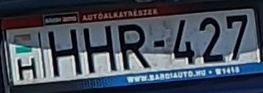
\includegraphics[width=\textwidth]{figures/preprocessbefore1.jpg}
    \end{subfigure}
    \hfill
    \begin{subfigure}[b]{.45\textwidth}
        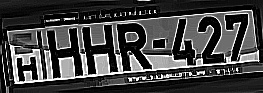
\includegraphics[width=\textwidth]{figures/preprocessafter1.jpg}
    \end{subfigure}
    \hfill
    \\
    \begin{subfigure}[b]{.45\textwidth}
        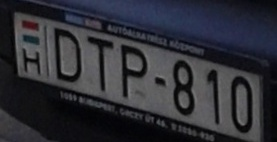
\includegraphics[width=\textwidth]{figures/preprocessbefore2.jpg}
    \end{subfigure}
    \hfill
    \begin{subfigure}[b]{.45\textwidth}
        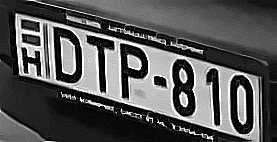
\includegraphics[width=\textwidth]{figures/preprocessafter2.jpg}
    \end{subfigure}
    \hfill
    \\
    \begin{subfigure}[b]{.45\textwidth}
        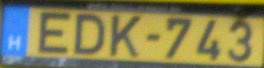
\includegraphics[width=\textwidth]{figures/preprocessbefore3.jpg}
    \end{subfigure}
    \hfill
    \begin{subfigure}[b]{.45\textwidth}
        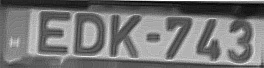
\includegraphics[width=\textwidth]{figures/preprocessafter3.jpg}
    \end{subfigure}
    \hfill
    \caption{Preprocessing results.}
    \label{fig:preprocessing-fig}
\end{figure}



\section{Evaluation}

\todo[inline]{Write this section, actualize it to what we actually did.}

\todo[inline]{Write about Precision/Recall, etc.}

We will consider different cases depending on the difficulty of the given image,
which will be determined based on how well our solution performs under
the given (visual) setting. Based on this, we will categorize these cases by
perceived difficulty, and show examples.

These are some of the settings we expect to make \ac{ALPR} more
difficult:\todo[inline]{Create these comparisons, plot them in a figure.}
\begin{itemize}
    \item Direct sunlight 
    \item Partial occlusion of the license plate 
    \item Miscellaneous weather effects such as rain or fog
    \item Small size of the licence plate (i.e. the object is further away)
\end{itemize}

We will examine which of these settings introduce the most perceived noise, thus
decreasing the effectiveness of our solution.

Other than these, -- as is the case with all learning-based methods, -- there is
an inherent uncertainty on the generalization capabilities of our solution.
After training and testing our solution on a predefined dataset, the real trial
will be generalizing to photos we never encountered, as these images will be
out-of-distribution for sure. Thus, we plan to finish our project with
evaluating our solution \textit{in the wild}, measuring its robustness on
real-life data.

\todo[inline]{Add image results.}



\newpage
\bibliography{literature.bib}
\newpage


\end{document}
